\documentclass[EEEE]{KGCOEReport}

\usepackage{biblatex}
\usepackage{graphicx}
\usepackage{newtxtext, newtxmath}
\usepackage{csquotes}
\usepackage{parskip}
\usepackage{karnaugh-map}
\usepackage{circuitikz}
\usepackage{float}
\usepackage{pdfpages}

\graphicspath{./assets/}
\addbibresource{./assets/bib.bib}

\newcommand{\classCode}{EEEE 281}
\newcommand{\className}{Circuits 1}

\newcommand{\name}{Aden Perry}
% \newcommand{\partnerName}{PARTNER}

\newcommand{\LabSectionNum}{L7}

\newcommand{\TAs}{Sol Holston}
\newcommand{\exerciseNumber}{1}
\newcommand{\exerciseDescription}{Voltage Divider}

\newcommand{\dateDone}{2026-02-19}
\newcommand{\dateSubmitted}{2026-02-17}


\begin{document}

\maketitle

\section*{Abstract}

The purpose of this exercise was to create a voltage divider to convert a
provided voltage to a given second voltage, using resistors in parallel.
An equation was derived to find the voltage across a given resistor for a
voltage source and two resistors connected in series. A second equation was
derived to find the voltage across a given resistor for a voltage source and
a resistor connected in series with two resistors in parallel. The derived
equations were used to find the resistance values required to convert a 5 volt
input to a 3.3 volt and 2.97 volt output. The resistance values were rounded
to standard manufacturer values, and the resultant circuit was simulated using
the LTspice simulation software. DC Bias point and Monte Carlo simulations
were conducted. Both circuits were implemented in hardware and tested uisng a
digital multimeter and a DC power source. The measured voltages matched the
simulated voltages, and the measured voltages were within a reasonable range of
the calculated voltages; the exercise was successful.

\section{Introduction and Theory}

The objective of this laboratory was to calculate the resistances, power losses
and gains, currents, and voltages in a voltage divider; to implement a voltage
divider in hardware; and to measure the output voltage.

\subsection{Theory: Circuits Investigated}

A circuit for a voltage divider is given in Figure \ref{fig:c1}.

\begin{figure}[H]
	\center
	\includegraphics{figures/circuit-1}
	\caption{Voltage divider circuit}
	\label{fig:c1}
\end{figure}

The circuit has a voltage source, $V_{in}$, and uses two resistors, $R_1$ and
$R_2$, connected in series to induce a voltage of $V_{out}$ across resistor
$R_2$. A current, $i$, flows through the circuit. It is useful to know how the
resistances and voltages influence each other in order to facilitate circuit
design. Equation \ref{equ:c1} expresses this relationship algebraically. The
derivation is shown below.

\begin{align*}
	V_{in}              & = R_1 i + R_2 i                                              \\
	R_2 i               & = V_{out}                                                    \\
	i                   & = \frac{V_{in} - V_{out}}{R_1}                               \\
	i                   & = \frac{V_{out}}{R_2}                                        \\
	\frac{V_{out}}{R_2} & = \frac{V_{in} - V_{out}}{R_1}                               \\
	0                   & = \frac{ R_2 V_{in} - R_2 V_{out} - R_1 V_{out} }{ R_1 R_2 } \\
	R_2 V_{in}          & = V_{out} (R_1 + R_2)
\end{align*}
\begin{equation}
	\boxed{V_{out} = V_{in} \frac{R_2}{R_1 + R_2}}
	\label {equ:c1}
\end{equation}

Equation \ref{equ:c1} was applied with a $V_{in}$ value of 5 volts, an $R_1$
value of 470 ohms, and a $V_{out}$ value of 3.3 volts. The equation was solved
for $R_2$ using a calculator, resulting in $R_2 = 912.353$ ohms. The closest
resistance readily available is 1000 ohms; thus, 1000 ohms was selected for
circuit simulation and implementation.

A circuit for a voltage divider with load is given in Figure \ref{fig:c2}.

\begin{figure}[H]
	\center
	\includegraphics{figures/circuit-2}
	\caption{Voltage divider with load}
	\label{fig:c2}
\end{figure}

The circuit is similar to the circuit described in Figure \ref{fig:c1}, with
the addition of a resistor, $R_L$, in parallel to the resistor $R_2$. A
current, $i_1$, flows through the resistor $R_1$. Currents $i_2$ and $i_L$ flow
through resistors $R_2$ and $R_L$, respectively. It is useful to know how the
resistances and voltages influence each other in order to facilitate circuit
design. Equation \ref{equ:c2} expresses this relationship algebraically. The
derivation is similar to that of Equation \ref{equ:c1}; the value of
$R_2 || R_L$ is equivalent to the value of $R_2$ in the latter equation. Thus,
Equation \ref{equ:c2} is found.

\begin{equation}
	\boxed{V_{out} = V_{in} \frac{ R_2 || R_L }{ R_1 + R_2 || R_L }}
	\label{equ:c2}
\end{equation}

Equation \ref{equ:c2} was applied with a $V_{in}$ value of 5 volts, an $R_1$
value of 470 ohms, an $R_2$ value of 1000 ohms, and a $V_{out}$ value of 2.97
volts (90\% of 3.3). The equation was solved for $R_L$ using a calculator,
resulting in $R_L = 2201.39$ ohms. The closest resistance readily available is
2200 ohms; thus, 2200 ohms was selected for circuit simulation and
implementation.

Using these values, Ohm's law was applied to determine that the power loss of
the voltage divider is 17.590 milliwatts, the power delivered to $R_{L}$ is
4.007 milliwatts, and the power generated by $V_{in}$ is 21.598 williwatts.

\subsection{Theory: LTspice Simulation}

The voltage divider circuit given in Figure \ref{fig:c1} was simulated in
LTspice. The schematic is shown in Figure \ref{fig:c1-schem}.

\begin{figure}[H]
	\center
	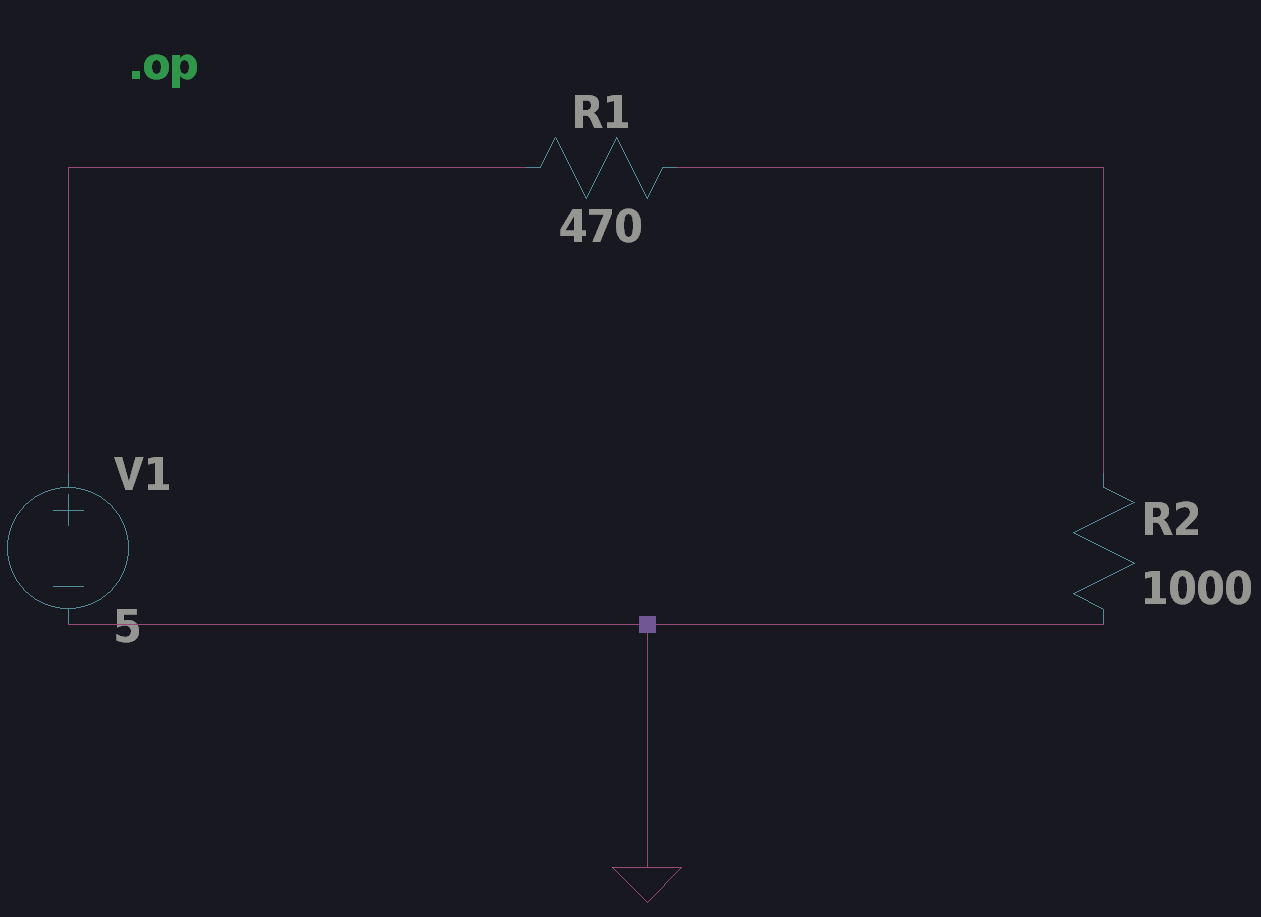
\includegraphics[width=0.5\textwidth]{assets/c1}
	\caption{Voltage divider in LTspice}
	\label{fig:c1-schem}
\end{figure}

LTspice was used to run a DC bias point simulation. The simulation determined
an expected $V_{out}$ of 3.4 volts. The discrepancy between the calculated
value and the simulated value is due to the rounding of $R_2$ to a commercially
available resistance.

The voltage divider circuit with a load given in Figure \ref{fig:c2} was
simulated in LTspice. The schematic is shown in Figure \ref{fig:c2-schem}.

\begin{figure}[H]
	\center
	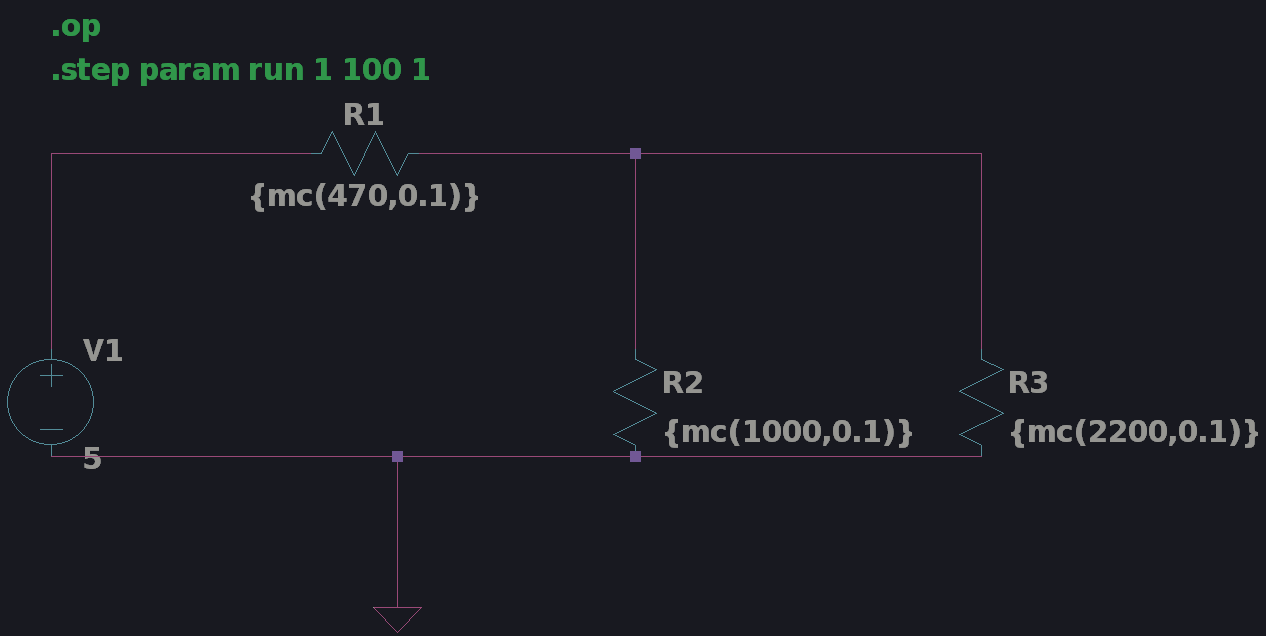
\includegraphics[width=0.5\textwidth]{assets/c2}
	\caption{Voltage divider with load in LTspice}
	\label{fig:c2-schem}
\end{figure}

LTspice was used to run a DC bias point simulation. The simulation determined
an expected $V_{out}$ of 2.9743 volts. The discrepancy between the calculated
value and the simulated value is due to the rounding of $R_L$ to a commercially
available resistance. Because the difference between the calculated value and
the available value is so small, it has little effect on the simulation
results.

A Monte Carlo simulation was performed on the voltage divider with a load. Each
resistor was given a 10\% tolerance, and 100 runs were performed. The results
are given in Figure \ref{fig:mc}.

\begin{figure}[H]
	\center
	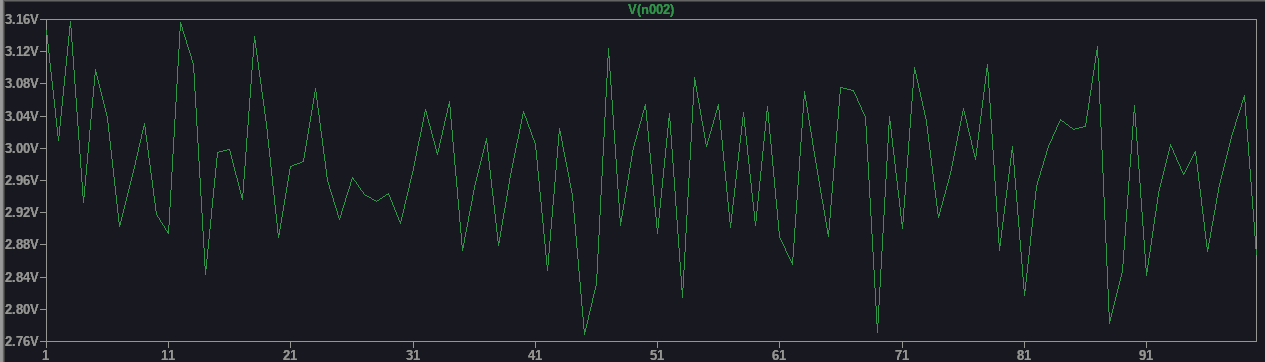
\includegraphics[width=\textwidth]{assets/monte-carlo}
	\caption{Results of Monte Carlo simulation}
	\label{fig:mc}
\end{figure}

In general, values for $V_{out}$ were near 2.97 volts. However, there was
significant variation. The largest simulated $V_{out}$ voltage was 3.16 volts.
The smallest simulated voltage was 2.76 volts.

\section{Hardware Experiment: Results and Discussion}

The circuit given by Figure \ref{fig:c1} was implemented in hardware. The
implementation is shown in Figure \ref{fig:c1-hw}.

\begin{figure}[H]
	\center
	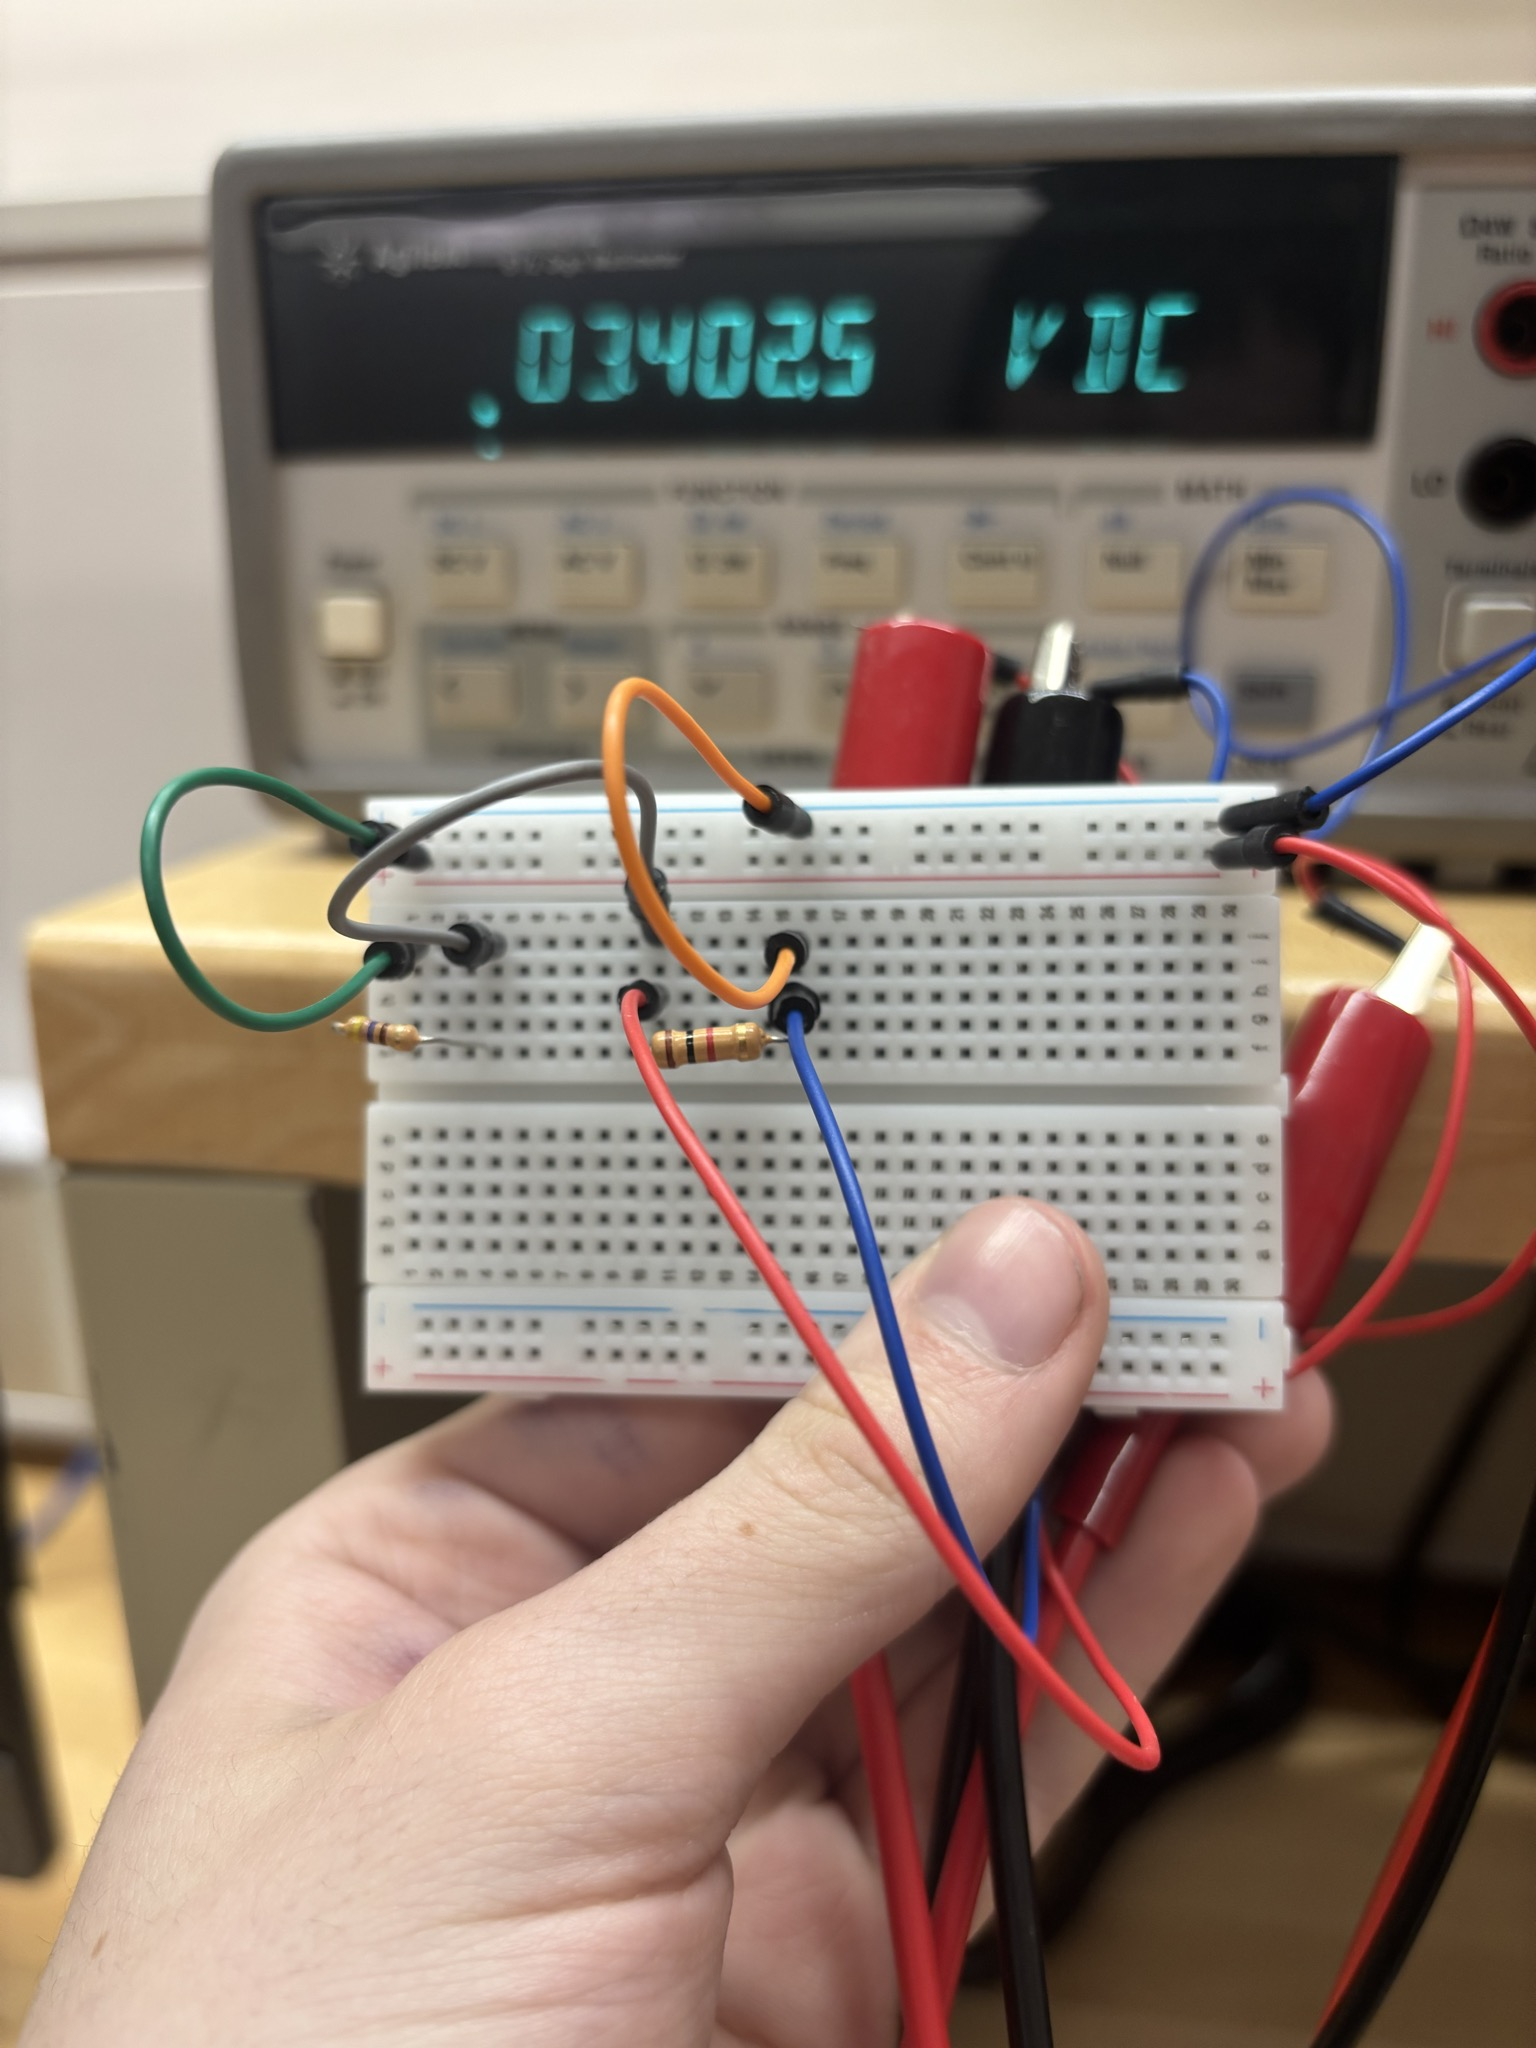
\includegraphics[width=0.5\textwidth]{assets/c1-hw}
	\caption{Implementation of voltage divider}
	\label{fig:c1-hw}
\end{figure}

The circuit was implemented on a breadboard. The rightmost red and blue wires
were connected to a 5 volt DC power source. The middle red and blue wires were
connected to a digital multimeter.

The circuit given by Figure \ref{fig:c2} was implemented in hardware. The
implementation is shown in Figure \ref{fig:c2-hw}.

\begin{figure}[H]
	\center
	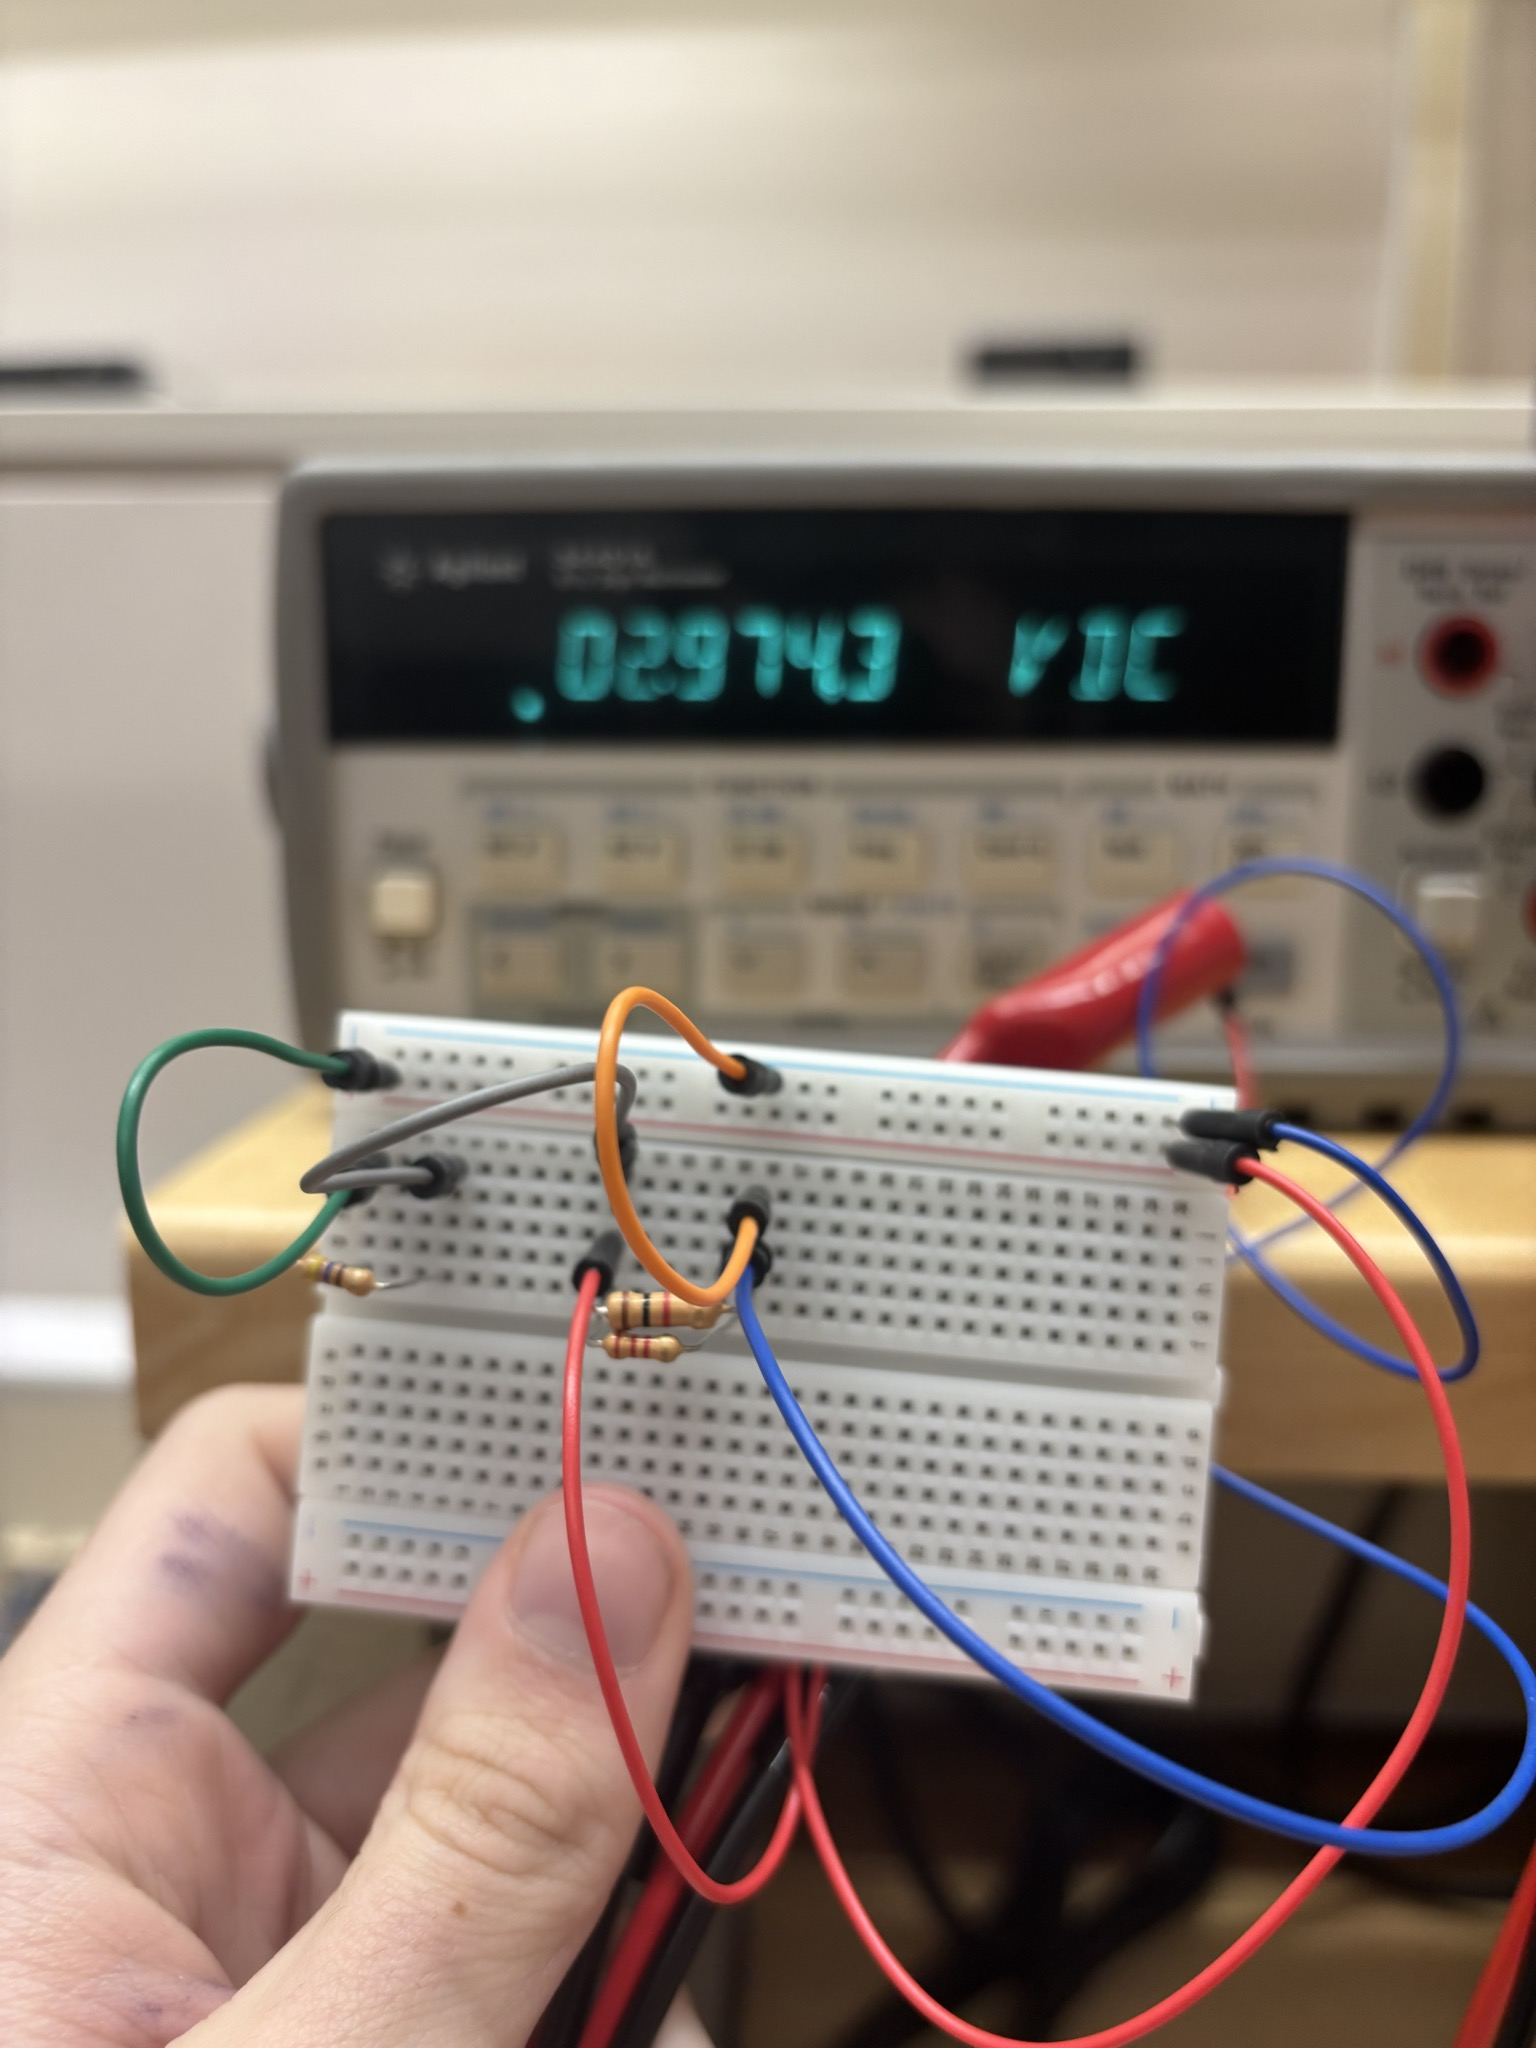
\includegraphics[width=0.5\textwidth]{assets/c2-hw}
	\caption{Implementation of voltage divider with load}
	\label{fig:c2-hw}
\end{figure}

The circuit was implemented on a breadboard. The rightmost red and blue wires
were connected to a 5 volt DC power source. The middle red and blue wires were
connected to a digital multimeter.

The measured voltages are visible in the background of Figures \ref{fig:c1-hw}
and \ref{fig:c2-hw}, and are also presented in Table \ref{tbl:hw-result}.

\begin{table}[H]
	\center
	\begin{tabular}{|c|c|}
		\hline
		                    & Voltage (V) \\
		\hline
		Circuit 1 $V_{out}$ & 3.4013      \\
		\hline
		Circuit 2 $V_{out}$ & 2.9743      \\
		\hline
	\end{tabular}
	\caption{Measured voltages}
	\label{tbl:hw-result}
\end{table}

The 3.4013 voltage from Circuit 1 has a 3.1\% error from the expected value of
3.3 volts. This is because a 1000 ohm resistor was used instead of a 912 ohm
resistor. A 3.1\% error is not especially significant.

The 2.9743 voltage from Circuit 2 has a 0.15\% error from the expected value of
2.97 volts. This is well within the range modeled by the Monte Carlo
simulation; there is exceptionally low error.

\section{Conclusion}

All results are provided in Table \ref{tbl:conc}.

\begin{table}[H]
	\center
	\begin{tabular}{|c|c|c|c|}
		\hline
		                        & Hand Calculation & Simulation & Hardware \\
		\hline
		Circuit 1 $V_{out}$ (V) & 3.3              & 3.4013     & 3.4025   \\
		\hline
		Circuit 2 $V_{out}$ (V) & 2.97             & 2.9743     & 2.9743   \\
		\hline
	\end{tabular}
	\caption{Final lab results}
	\label{tbl:conc}
\end{table}

The differences between the calculated, simulated, and measured voltages in
Circuits 1 and 2 can be used to determine that a high load will decrease the
output voltage of a voltage divider.

\section{Acknowledgements}

Methods described in the textbook \textit{Fundamentals of Electric Circuits,
	7th Ediition} \cite{fec} were used to derive Equations \ref{equ:c1} and
\ref{equ:c2}.

The template for this Technical Memo was modified from a \LaTeX \ class created
by Joshua Milas and Seth Gower, using the provided Tech Memo Template and
example Tech Memo from the Advanced Course as inspiration.

\printbibliography

\end{document}
